\documentclass[a4paper, 11pt]{article}
\usepackage{comment} % enables the use of multi-line comments (\ifx \fi) 
\usepackage{fullpage} % changes the margin
\usepackage[margin=35pt]{geometry}
\usepackage{graphicx}
\usepackage{microtype} 
\usepackage{titlesec}
\usepackage{color, colortbl}
\usepackage[table]{xcolor} 
%\usepackage[most]{tcolorbox}

%\usepackage{fontspec}
%\setmainfont{Georgia} 
\titleformat*{\section}{\large\bfseries}

\begin{document}

\noindent
\large\textbf{Committee Meeting Report} \hfill \textbf{Sahar Mozaffari} \\
\normalsize  \hfill Professor: Carole Ober  \\
GGSB Matriculated 2013 \hfill Date: 09/08/16 \\
\noindent\makebox[\linewidth]{\rule{\paperwidth}{0.4pt}}

\large\textbf{\\Progress since last Committee Meeting - June 16, 2015}
\subsection*{Awards}
% Horizontal line after name; adjust line thickness by changing the '1pt'
\begin{itemize}
    \item Awarded F31 Ruth L. Kirschstein NRSA 
    \item FASEB MARC Travel Award to ASHG 2015 in Baltimore, MD
    \item FASEB MARC Travel Award to ASHG 2014 in San Diego, CA
    \item Genetics and Regulation Training Grant: 2013-2016
\end{itemize} 

\subsection*{Publications}
\begin{itemize}
    \item Gamazon, E. R., Wheeler, H. E., Shah, K. P., Mozaffari, S. V., Aquino-Michaels, K., Carroll, R. J., et al. (2015). \emph{A gene-based association method for mapping traits using reference transcriptome data.} Nature Genetics, 47(9), 1091–1098. http://doi.org/10.1038/ng.3367\cite{Gamazon}
\end{itemize}

\subsection*{Presentations}
\begin{itemize}
	\item Genetics of Model Organisms Club \hfill April 21, 2016\\
	Mozaffari, SV. \emph{Parent of Origin Effects in the Hutterites}
    \item Complex Trait Mapping Journal Club \hfill March 25, 2016\\
    Paper: Amin V, Harris RA, Onuchic V, et al. \emph{Epigenomic footprints across 111 reference epigenomes reveal tissue-specific epigenetic regulation of lincRNAs.} Nat Commun. 2015;6:6370.
	\item Human Genetics Work in Progress \hfill January 20, 2016\\
    		Mozaffari, SV. \emph{Parent of Origin Effects} 
	\item Molecular Biosciences Retreat \hfill November 5, 2015\\ Mozaffari SV, DeCara J, Shah S, Herman C, Lang R, Nicolae D, Ober C., \emph{Parent of Origin GWAS with Cardiovascular Disease Associated Traits in the Hutterites.} 2015: Nov 5; Galena, IL.
    \item ASHG\hfill October 9, 2015\\ Mozaffari SV, DeCara J, Shah S, Herman C, Lang R, Nicolae D, Ober C., \emph{Parent of Origin GWAS of CVD-Associated Phenotypes in the Hutterites} (Abstract Program \#310). Presented at the Annual Meeting of The American Society of Human Genetics; 2015: Oct 9; Baltimore, MD. 
  

\end{itemize}

\subsection*{Posters}
\begin{itemize}
    \item Mozaffari SV, Gamazon E, Aquino-Michaels K, Cox NJ, Im HK. \emph{Quantifying Context Specificity of Gene Regulation using Predicted Gene Expression Levels.} Poster presented at the Annual Meeting of The American Society of Human Genetics Conference; 2014: Oct 18-22; San Diego, CA 
\end{itemize}

\subsection*{Teaching Assistantship Requirements Completed}
\begin{itemize}
    \item MGCB 31400 (BIOS 21236) \emph{Genetic Analysis of Model Organisms}\hfill Fall 2014\\
Graduate \& Undergraduate Course: Introduction to genetic tools, experiments, and model organisms 

	\item HGEN 47000 \emph{Human Genetics} \hfill Fall 2015\\
Graduate Course: Classic and modern approaches to studying cytogenetic, Mendelian, and complex human diseases. Grant proposal writing course. 
\end{itemize}


\subsection*{Additional Courses}
\begin{itemize}
    \item STAT 24500 \emph{Statistical Theory \& Methods II }\hfill Winter 2015
    \item HGEN 46900 \emph{Human Variation \& Disease} \hfill Spring 2015
    \item STAT 35500 \emph{Statistical Genetics} \hfill Spring 2015
    \item myChoice Mini-Course: \emph{Effective Writing in the Biological Sciences} \hfill Fall 2015
    \item HGEN 48600 \emph{Fundamentals of Computational Biology: Models \& Inference} \hfill Winter 2016
    \item PBHS 31831 \emph{Genetic \& Molecular Epidemiology} \hfill Spring 2016
  
	
\end{itemize}

\subsection*{Additional Workshops}
\begin{itemize}
   \item Master R Developer Workshop taught by Hadley Wickham \hfill May 2015
     \item Summer Institute in Statistical Genetics at the University of Washington \hfill July 2016
\end{itemize}

\subsection*{Extracurricular}
\begin{itemize}
	\item Museum of Science \& Industry: Science Connections volunteer \hfill Fall 2014-current
    \item myCHOICE Internship: Institute of Translational Medicine \hfill Summer 2015\\Translate complex research into dynamic science stories. Share translational research stories in weekly newsletter, ITM website, and social media platforms

\end{itemize}



%\noindent\makebox[\linewidth]{\rule{\paperwidth}{0.4pt}}

%\section*{Attachments}
%Make sure to change these
%Lab Notes, HelloWorld.ic, FooBar.ic
%\fi %comment me out
\newpage

%\noindent\makebox[\linewidth]{\rule{\paperwidth}{0.4pt}}
\section*{Proposal Updates:}
%\begin{tcolorbox}[colback=white,colframe=red!75!black]
I would like to revise my aims to focus on Parent of Origin Effects. There are many different aspects of the project to explore and I would like to take advantage of it. These were my previous aims.

\textbf{\\AIM 1} To identify and characterize parent of origin effects and allele specific effects on gene expression in 430 Hutterites.\\
\textbf{AIM 2} To investigate association of gene age and eQTLs in endometrial-expressed genes in humans.\\
\textbf{AIM 3} To characterize the contributions of genetic variants, IBD segments, parent of origin, functional variants, and relatedness among individuals to predict clinical phenotypes.\\

The following are my proposed revised aims:

\textbf{\\AIM 1a} To identify and characterize parent of origin effects on quantitative traits in the Hutterites. 
   \textbf{\\AIM 1b} To estimate maternal and paternal heritability measures on quantitative traits in the Hutterites.
\textbf{\\AIM 2a} To identify and characterize parent of origin effects on gene expression in 430 Hutterites.\\
\textbf{AIM 2b} To identify and characterize parent of origin and allele specific effects on gene expression in 430 Hutterites.\\



Previously, I shared results on parent of effects on gene expression where I tested maternally- and paternally- inherited alleles separately with the sum of gene expression.\cite{Cusanovich} I received feedback to separate the gene expression into reads that map maternally and those that map paternally, and to use these measures for POeQTL.

\textbf{\\Since my Qualifying Exam}

\textbf{\\AIM 1}\\
I have ran Parent of Origin GWAS, testing maternally and paternally- inherited alleles separately with 22 different traits. The manhattan plots for the Maternal and Paternal GWAS for LDL are in Figure 1. Table 1 has the phenotypes with significant maternal and paternal allele associations. \\

\begin{figure}[!h]
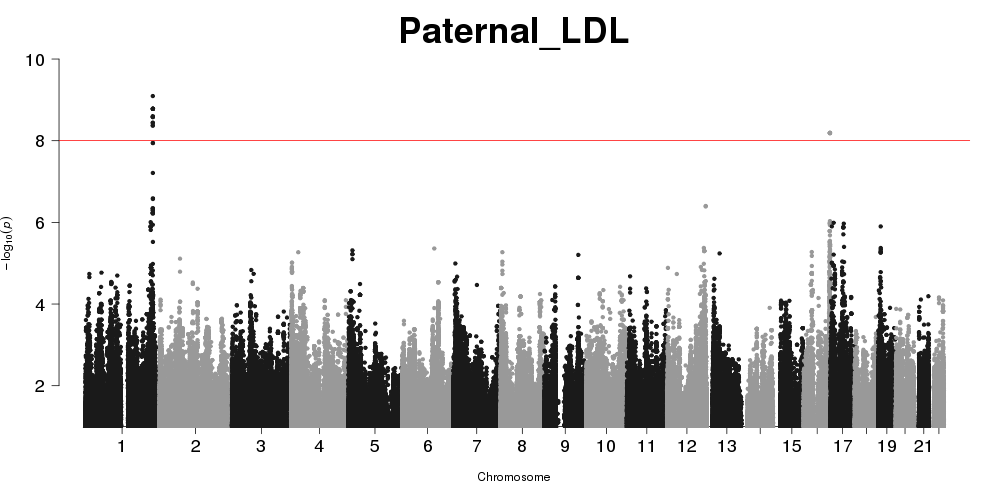
\includegraphics[width=0.5\textwidth]{Manhattan_paternal_LDL_8_17_16.png}
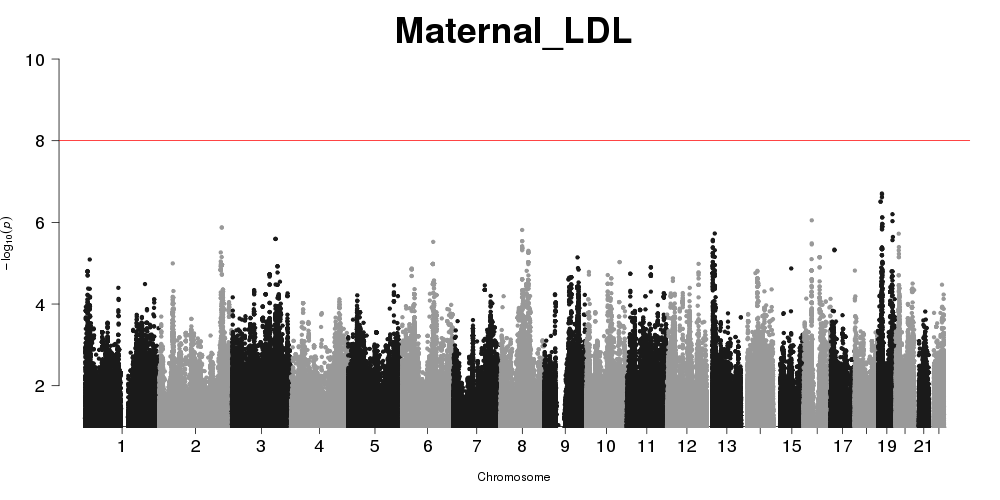
\includegraphics[width=0.5\textwidth]{Manhattan_maternal_LDL_8_17_16.png}
\caption{\label{fig:POGWAS}Paternal and Maternal allele PO- GWAS Manhattan plots for LDL.}
\end{figure}

\begin{table}[!h]
\begin{centering}
\begin{tabular}{lll} \hline
& Phenotypes \\ \hline
Significant Maternal Association & Carotid Intima Media Thickness, FEV\textsubscript{1}, Trigylcerides \\ \hline
Significant Paternal Associations & Systolic Blood Pressure, Blood eosinophil count LDL-C \\ &  Total cholesterol\\ \hline
No Significant Parental Associations & Left Atrial Volume Index, Left Ventricular Mass Index, FEV\textsubscript{1}/FVC,  \\ &  Bronchial Responsiveness Index, Fraction exhaled nitric oxide \\
& Diastolic Blood Pressure, Lymphocyte Count, Monocyte Count, \\
& Neutrophil Count, IgE, Chitin, YKL40, BMI, Height, HDL-C \  \\ \hline 
\end{tabular}
\caption{\label{tab:Signif}Phenotypes with Significant Maternal or Paternal Allele Associations.}
\end{centering}
\end{table}
\newpage
I have also ran a new model (equation 1) that tests for difference of parental effects in two of these phenotypes (LDL \& BMI), and I am working on running them on the remaining 20 phenotypes. I  am working on replicating the interesting findings with BMI in the Framingham cohort.\\
\begin{equation}\label{my_first_eqn}
	Y=\mu + (\beta_p-\beta_m)\frac{(X_p-X_m)}{2} +\frac{(\beta_p+\beta_m)}{2}X_{mp} + \epsilon
\end{equation}
 \textbf{AIM 1b}\\With the help of Mark Abney, I have models to test for parent of origin heritability. I have estimated the average maternal and average paternal heritability for each of the 22 traits and I am working on getting a more accurate measure (as opposed to average).\\
\textbf{\\AIM 2a}\\
I have remapped the LCL RNA-seq data using STAR\cite{Dobin} and corrected sample swaps using verifyBamID (fixed 2 samples that were already included, and gained 4 samples).\cite{Jun} I used WASP\cite{van de Geijn} to remove mapping bias and mapped reads to the maternal and paternal haplotypes.\\
\\For this aim I have methods to detect patterns of parent of origin effects (i.e. imprinting) using maternal and paternal gene expression but not any SNPs (no POeQTL). First I test for asymmetry in maternal and paternal gene expression (normalized total gene expression) with permutations of the data. The second test uses a binomial test to get a Z-score of maternal and paternal expression within each sample (not normalized gene expression). The distribution of the Z-score can be tested against a normal distribution with the Shapiro-Wilk test. The most significant genes from this test have a lot of overlap with known imprinted genes as shown in Table 2 \& 3. 

%\begin{table}[!h]
%\begin{centering}
%\begin{tabular}{l|l|l} 
%Predicted Paternally Imprinted & Imprinted & Shapiro-Wilk p-value \\ \hline
%CACNA2D1 & no & \\ \hline
%UNC93B1 & no & \\ \hline

%\end{tabular}
%\caption{\label{tab:Genes}Significant Genes that have Parent of Origin effects}
%\quad
%\end{centering}
%\end{table}

\definecolor{lavender}{RGB}{230,230,250}
\definecolor{mistyrose}{RGB}{255,228,225}

\begin{table}[!ht]
\parbox{.45\linewidth}{
\begin{tabular}{l|lll}
Gene & Imprinted & Asymmetry & Shapiro \\ \hline
\emph{CACNA2} & no & 0 & 0.58 \\ \hline
\emph{UNC93B1} & no &  0 & 0.72\\ \hline
\emph{HCAR2} & no &  0 & NA\\ \hline
\emph{CTAGE10} & no &  0 & 5e\textsuperscript{-08}\\ \hline
\emph{MTRNR2} & no & 0 & 0.46\\ \hline
\emph{CRYBB2P} & no &  0 & 0.18 \\ \hline
\rowcolor{mistyrose}
\emph{H19} & yes &  0 & 1.57e\textsuperscript{-08}\\ \hline
\emph{SUPT4H1} & no &  0 & 0.75\\ \hline
\emph{EIF4A3} & no &  0 & 0.14\\ \hline
\rowcolor{mistyrose}
\emph{ZNF597} & yes &  0 &5.63e\textsuperscript{-13}\\ \hline
\emph{DIDO1} & no &  0 & 1.05e\textsuperscript{-03}\\ \hline
\emph{EIF2AK1} & no &  0 & 0.12\\ \hline
\emph{LOC38897} & no & 0 & 1.65e\textsuperscript{-08}\\ \hline
\rowcolor{mistyrose}
\emph{KCNQ1} & yes &  0 & 0 \\ \hline
\emph{SEC61A1} & no &  0 & 2.43e\textsuperscript{-06}\\ \hline
\emph{CPNE1} & no &  0 & 0\\ \hline
\emph{SEC22B} & no &  0 & 0\\ \hline


\end{tabular}
\caption{\label{tab:PaternalGenes} Paternally Imprinted  (maternally expressed) genes significant from the Asymmetry test (p-values in column 3); top 17 genes with p-value 0. Known imprinting status in column 2, and Shapiro test p-value in column 4. Colored in pink are known paternally imprinted genes from geneimprint.com.}
}
\quad
\parbox{.45\linewidth}{

%\begin{centering}
\begin{tabular}{l|lll}
Gene & Imprinted & Asymmetry & Shapiro \\ \hline

\rowcolor{lavender}
\emph{MEST} & yes & 0 & 2.3e\textsuperscript{-07}\\ \hline

\emph{MRPL28} & no & 0 & 0.13\\ \hline
\rowcolor{lavender}
\emph{BMP8A} & yes & 0 &3.67e\textsuperscript{-06}\\ \hline
\emph{EIF5AL1} & no & 0 &0.08\\ \hline
\rowcolor{lavender}
\emph{FAM50B} & yes & 0 & 6.05e\textsuperscript{-12}\\ \hline
\emph{PRIM2} & conflicting & 0 & 0.72\\ \hline
\emph{TCEA1} & no & 0 & 0.02\\ \hline
\emph{LPAR6} & no &0 & 3.65e\textsuperscript{-05}\\ \hline
\emph{PCGF5} & no & 0 &2.18e\textsuperscript{-17}\\ \hline
\emph{DUSP22} & no & 0 & 0.24\\ \hline
\emph{ZNF331} & no & 0 & 0.24\\ \hline
\rowcolor{lavender}
\emph{NHP2L1} & yes & 0 & 3.13e\textsuperscript{-05}\\ \hline
\rowcolor{lavender}
\emph{ZDBF2} & yes & 0 &1.31e\textsuperscript{-09}\\ \hline
\rowcolor{lavender}
\emph{PEG10} & yes & 0 &2.29e\textsuperscript{-10}\\ \hline
\emph{TMEM30A} & no & 0 & 0.98\\ \hline
\emph{BCLAF1} & no & 0 &1.5e\textsuperscript{-04}\\ \hline
\emph{MAP2K3} & no & 0 & 7.2e\textsuperscript{-13}\\ \hline
\end{tabular}
\caption{\label{tab:MaternalGenes} Maternally Imprinted  (paternally expressed) genes significant from the Asymmetry test (p-values in column 3); top 17 genes with p-value 0. Known imprinting status in column 2, and Shapiro test p-value in column 4. Colored in blue are known maternally imprinted genes from geneimprint.com.}
}
\quad

\end{table}
\begin{flushleft}
\textbf{AIM 2b}\\
I will test for POeQTLs in this aim testing maternally inherited SNPs with the maternal gene expression and paternally inherited SNPs with paternal expression. I will combine this with POeQTL results from before using the sum of gene expression, especially for genes which we don't have maternal or paternal expression.
\end{flushleft}
%\end{tcolorbox}
\begin{thebibliography}{9}
\bibitem{Gamazon} Gamazon, E. R., Wheeler, H. E., Shah, K. P., Mozaffari, S. V., Aquino-Michaels, K., Carroll, R. J., et al. (2015). A gene-based association method for mapping traits using reference transcriptome data. Nature Genetics, 47(9), 1091–1098. http://doi.org/10.1038/ng.3367
\bibitem{Cusanovich} Cusanovich, D. A., Caliskan, M., Billstrand, C., Michelini, K., Chavarria, C., De Leon, S., et al. (2016). Integrated analyses of gene expression and genetic association studies in a founder population. Human Molecular Genetics, ddw061. http://doi.org/10.1093/hmg/ddw061
\bibitem{Dobin} Dobin, A., \& Gingeras, T. R. (2015). Mapping RNA-seq Reads with STAR. Current Protocols in Bioinformatics. 51, 11.14.1–19. http://doi.org/10.1002/0471250953.bi1114s51
\bibitem{Jun} G. Jun, M. Flickinger, K. N. Hetrick, Kurt, J. M. Romm, K. F. Doheny, G. Abecasis, M. Boehnke,and H. M. Kang, (2012) Detecting and Estimating Contamination of Human DNA Samples in Sequencing and Array-Based Genotype Data, AJHG doi:10.1016/j.ajhg.2012.09.004 (volume 91 issue 5 pp.839 - 848)
\bibitem{van de Geijn}van de Geijn B, McVicker G, Gilad Y, Pritchard JK. (2015) WASP: allele-specific software for robust molecular quantitative trait locus discovery. Nat Meth. 12:1061-1063. doi:10.1038/nmeth.3582.
\end{thebibliography}

\end{document}
